\documentclass[UTF8]{ctexart}
\usepackage[UTF8]{ctex}
\usepackage{listings}
\usepackage{xcolor}
\usepackage{graphicx}
\usepackage{appendix}

%代码段设置
\lstset{numbers=left,
basicstyle=\tiny,
numberstyle=\tiny,
keywordstyle=\color{blue!70},
commentstyle=\color{red!50!green!50!blue!50},
frame=single, rulesepcolor=\color{red!20!green!20!blue!20},
escapeinside=``
}

\graphicspath{ {../Gan/gan_project/images/}{../Gan/cnn_project/improved_images/} }
\usepackage{graphicx}
\usepackage{color,framed}%文本框
\usepackage{listings}
\usepackage{caption}
\usepackage{amssymb}
\usepackage{enumerate}
\usepackage{xcolor}
\usepackage{bm} 
\usepackage{lastpage}%获得总页数
\usepackage{fancyhdr}
\usepackage{tabularx}  
\usepackage{geometry}
\usepackage{minted}
\usepackage{graphics}
\usepackage{subfigure}
\usepackage{float}
\usepackage{pdfpages}
\usepackage{pgfplots}
\pgfplotsset{width=10cm,compat=1.9}
\usepackage{multirow}
\usepackage{footnote}
\usepackage{booktabs}

%-----------------------伪代码------------------
\usepackage{algorithm}  
\usepackage{algorithmicx}  
\usepackage{algpseudocode}  
\floatname{algorithm}{Algorithm}  
\renewcommand{\algorithmicrequire}{\textbf{Input:}}  
\renewcommand{\algorithmicensure}{\textbf{Output:}} 
\usepackage{lipsum}  
\makeatletter
\newenvironment{breakablealgorithm}
  {% \begin{breakablealgorithm}
  \begin{center}
     \refstepcounter{algorithm}% New algorithm
     \hrule height.8pt depth0pt \kern2pt% \@fs@pre for \@fs@ruled
     \renewcommand{\caption}[2][\relax]{% Make a new \caption
      {\raggedright\textbf{\ALG@name~\thealgorithm} ##2\par}%
      \ifx\relax##1\relax % #1 is \relax
         \addcontentsline{loa}{algorithm}{\protect\numberline{\thealgorithm}##2}%
      \else % #1 is not \relax
         \addcontentsline{loa}{algorithm}{\protect\numberline{\thealgorithm}##1}%
      \fi
      \kern2pt\hrule\kern2pt
     }
  }{% \end{breakablealgorithm}
     \kern2pt\hrule\relax% \@fs@post for \@fs@ruled
  \end{center}
  }
\makeatother
%------------------------代码-------------------
\usepackage{xcolor} 
\usepackage{listings} 
\lstset{ 
breaklines,%自动换行
basicstyle=\small,
escapeinside=``,
keywordstyle=\color{ blue!70} \bfseries,
commentstyle=\color{red!50!green!50!blue!50},% 
stringstyle=\ttfamily,% 
extendedchars=false,% 
linewidth=\textwidth,% 
numbers=left,% 
numberstyle=\tiny \color{blue!50},% 
frame=trbl% 
rulesepcolor= \color{ red!20!green!20!blue!20} 
}

%-------------------------页面边距--------------
\geometry{a4paper,left=2.3cm,right=2.3cm,top=2.7cm,bottom=2.7cm}
%-------------------------页眉页脚--------------
\usepackage{fancyhdr}
\pagestyle{fancy}
\lhead{\kaishu \leftmark}
% \chead{}
\rhead{\kaishu 生成对抗网络实验报告}%加粗\bfseries 
\lfoot{}
\cfoot{\thepage}
\rfoot{}
\renewcommand{\headrulewidth}{0.1pt}  
\renewcommand{\footrulewidth}{0pt}%去掉横线
\newcommand{\HRule}{\rule{\linewidth}{0.5mm}}%标题横线
\newcommand{\HRulegrossa}{\rule{\linewidth}{1.2mm}}
\setlength{\textfloatsep}{10mm}%设置图片的前后间距
%--------------------文档内容--------------------

\begin{document}
\renewcommand{\contentsname}{目\ 录}
\renewcommand{\appendixname}{附录}
\renewcommand{\appendixpagename}{附录}
\renewcommand{\refname}{参考文献} 
\renewcommand{\figurename}{图}
\renewcommand{\tablename}{表}
\renewcommand{\today}{\number\year 年 \number\month 月 \number\day 日}

%-------------------------封面----------------
\begin{titlepage}
    \begin{center}
    
\includegraphics[width=0.8\textwidth]{NKU.png}\\[1cm]
    \vspace{20mm}
		\textbf{\huge\textbf{\kaishu{计算机学院}}}\\[0.5cm]
		\textbf{\Huge\textbf{\kaishu{生成对抗网络实验报告}}}

		\vspace{\fill}
    \centering
    \textsc{\LARGE \kaishu{姓名\ :\ 钟坤原}}\\[0.5cm]
    \textsc{\LARGE \kaishu{学号\ :\ 2212468}}\\[0.5cm]
    \textsc{\LARGE \kaishu{专业\ :\ 计算机科学与技术}}\\[0.5cm]
    \vfill
    {\Large }
    \end{center}
\end{titlepage}

\renewcommand {\thefigure}{\thesection{}.\arabic{figure}}%图片按章标号
\renewcommand{\figurename}{图}
\renewcommand{\contentsname}{目录}  
\cfoot{\thepage\ of \pageref{LastPage}}%当前页 of 总页数

% 生成目录
\clearpage
\tableofcontents
\newpage

%--------------------------摘要-------------------------------
\section*{摘要}
\addcontentsline{toc}{section}{摘要}
本实验报告详细介绍了生成对抗网络(GAN)的基本原理和实现过程。通过使用PyTorch框架,我们实现了原始GAN和深度卷积生成对抗网络(DCGAN)两种模型,并在FashionMNIST数据集上进行了训练和评估。实验包括了网络架构设计、训练过程分析、生成图像质量评估以及潜在空间的探索。结果表明,DCGAN相比原始GAN在图像生成质量和训练稳定性方面都有显著提升,卷积结构能够更好地捕捉图像的空间特征,生成更加逼真的时尚服装图像。

\textbf{关键词:}生成对抗网络;深度卷积生成对抗网络;FashionMNIST;图像生成;潜在空间

%--------------------------引言-------------------------------
\section{引言}
\addcontentsline{toc}{section}{引言}

生成对抗网络(Generative Adversarial Networks, GAN)是由Ian Goodfellow等人在2014年提出的一种深度学习模型,它通过两个神经网络的对抗训练来学习数据分布并生成新的数据样本。GAN的核心思想是让生成器(Generator)和判别器(Discriminator)进行博弈:生成器试图生成足够逼真的假数据来欺骗判别器,而判别器则努力区分真实数据和生成的假数据。

随着深度学习技术的发展,GAN在图像生成、数据增强、风格迁移等领域取得了显著成果。特别是深度卷积生成对抗网络(DCGAN)的提出,通过引入卷积神经网络结构,大大提升了图像生成的质量和训练的稳定性。

本实验旨在通过实现和比较原始GAN和DCGAN模型,深入理解生成对抗网络的工作原理,分析不同网络架构对生成效果的影响,并探索潜在空间的特性。实验使用FashionMNIST数据集,该数据集包含10类时尚服装图像,为评估模型的生成能力提供了良好的基准。

%--------------------------理论基础-------------------------------
\section{理论基础}

\subsection{生成对抗网络(GAN)}

生成对抗网络由两个神经网络组成:生成器$G$和判别器$D$。生成器$G$的目标是从随机噪声$z$中生成逼真的数据样本$G(z)$,而判别器$D$的目标是区分真实数据$x$和生成的假数据$G(z)$。

GAN的训练过程可以表示为以下的极小极大博弈问题:
\begin{equation}
\min_G \max_D V(D,G) = \mathbb{E}_{x \sim p_{data}(x)}[\log D(x)] + \mathbb{E}_{z \sim p_z(z)}[\log(1-D(G(z)))]
\end{equation}

其中:
\begin{itemize}
\item $p_{data}(x)$是真实数据分布
\item $p_z(z)$是输入噪声分布(通常为高斯分布)
\item $D(x)$表示判别器认为$x$为真实数据的概率
\item $G(z)$表示生成器从噪声$z$生成的数据
\end{itemize}

\subsection{深度卷积生成对抗网络(DCGAN)}

DCGAN是GAN在卷积神经网络上的扩展,主要改进包括:

\begin{enumerate}
\item \textbf{网络架构}:使用卷积和转置卷积层替代全连接层
\item \textbf{批归一化}:在生成器和判别器中使用批归一化层
\item \textbf{激活函数}:生成器使用ReLU激活函数,输出层使用Tanh;判别器使用LeakyReLU
\item \textbf{池化层}:使用步长卷积替代池化层
\end{enumerate}

这些改进使得DCGAN在图像生成任务上表现更加稳定和高效。

\subsection{卷积实现生成器和判别器的原理}

卷积神经网络在图像处理任务中具有天然的优势,其在GAN中的应用主要体现在以下几个方面:

\subsubsection{卷积生成器的设计原理}

卷积生成器通过转置卷积(反卷积)操作将低维的噪声向量逐步上采样为高分辨率图像:

\begin{enumerate}
\item \textbf{转置卷积层}:使用\texttt{ConvTranspose2d}将特征图尺寸逐步放大
\begin{itemize}
\item 第一层:将100维噪声向量reshape为$(100, 1, 1)$,通过转置卷积扩展到$(512, 4, 4)$
\item 后续层:依次将特征图尺寸从$4 \times 4$扩展到$7 \times 7$、$14 \times 14$、$28 \times 28$
\item 最终层:使用普通卷积将通道数从64降到1,保持$28 \times 28$的图像尺寸
\end{itemize}

\item \textbf{批归一化}:在每个转置卷积层后添加\texttt{BatchNorm2d},稳定训练过程
\begin{itemize}
\item 规范化特征分布,防止梯度消失或爆炸
\item 允许使用更高的学习率,加速收敛
\item 减少对权重初始化的敏感性
\end{itemize}

\item \textbf{激活函数选择}:
\begin{itemize}
\item 隐藏层使用ReLU激活函数,保持梯度流动
\item 输出层使用Tanh激活函数,将输出限制在$[-1, 1]$区间
\end{itemize}
\end{enumerate}

\subsubsection{卷积判别器的设计原理}

卷积判别器通过标准卷积操作将输入图像逐步下采样并提取特征:

\begin{enumerate}
\item \textbf{卷积层设计}:使用步长为2的卷积核实现下采样
\begin{itemize}
\item 第一层:$(1, 28, 28) \rightarrow (64, 14, 14)$
\item 第二层:$(64, 14, 14) \rightarrow (128, 7, 7)$
\item 第三层:$(128, 7, 7) \rightarrow (256, 3, 3)$
\item 输出层:$(256, 3, 3) \rightarrow (1, 1, 1)$
\end{itemize}

\item \textbf{正则化技术}:
\begin{itemize}
\item 使用\texttt{Dropout2d}防止过拟合,提高泛化能力
\item 在除第一层外的所有层使用批归一化
\item LeakyReLU激活函数避免神经元死亡问题
\end{itemize}

\item \textbf{特征提取机制}:
\begin{itemize}
\item 浅层提取低级特征(边缘、纹理)
\item 深层提取高级语义特征(形状、结构)
\item 最终输出单一概率值表示真实性判断
\end{itemize}
\end{enumerate}

\subsubsection{卷积架构的优势}

相比全连接网络,卷积架构在GAN中具有以下优势:

\begin{itemize}
\item \textbf{参数效率}:通过权重共享大幅减少参数数量
\item \textbf{空间不变性}:卷积操作保持图像的空间结构信息
\item \textbf{层次特征学习}:从低级到高级的渐进式特征提取
\item \textbf{训练稳定性}:批归一化和适当的网络深度提高训练稳定性
\item \textbf{生成质量}:更好地捕捉图像的局部和全局特征
\end{itemize}

%--------------------------实验设计-------------------------------
\section{实验设计}

\subsection{数据集}

本实验使用FashionMNIST数据集,该数据集包含:
\begin{itemize}
\item 训练集:60,000张28×28像素的灰度图像
\item 测试集:10,000张28×28像素的灰度图像
\item 类别:10类时尚服装(T恤、裤子、套衫、连衣裙、外套、凉鞋、衬衫、运动鞋、包、短靴)
\end{itemize}

数据预处理包括:
\begin{itemize}
\item 将像素值归一化到[-1, 1]区间
\item 转换为PyTorch张量格式
\item 设置批次大小为64
\end{itemize}

\subsection{模型架构}

\subsubsection{模型架构概述}

本实验实现了三种不同的GAN架构:

\textbf{原始GAN:}
采用全连接层构建生成器和判别器,生成器将100维噪声向量通过多层全连接网络映射为784维图像向量,判别器则将图像向量映射为真实性概率。

\textbf{DCGAN:}
使用卷积神经网络架构,生成器采用转置卷积层进行上采样,判别器使用标准卷积层进行下采样,并加入批归一化技术提升训练稳定性。

\textbf{改进卷积GAN:}
在DCGAN基础上进行优化,采用更深的网络结构和改进的权重初始化策略,提升生成图像质量和训练收敛性。

详细的模型架构实现请参见附录中的代码部分。

\subsection{训练参数}

\begin{table}[H]
\centering
\caption{训练参数设置}
\begin{tabular}{|c|c|c|c|}
\hline
\textbf{参数} & \textbf{原始GAN} & \textbf{DCGAN} & \textbf{改进卷积GAN} \\
\hline
学习率 & 0.0002 & 0.0002 & 0.0002 \\
\hline
Beta1 & 0.5 & 0.5 & 0.5 \\
\hline
Beta2 & 0.999 & 0.999 & 0.999 \\
\hline
批次大小 & 64 & 64 & 64 \\
\hline
训练轮数 & 50 & 50 & 50 \\
\hline
优化器 & Adam & Adam & Adam \\
\hline
损失函数 & BCELoss & BCELoss & BCELoss \\
\hline
Dropout比例 & 0.3 & 0.3 & 0.3 \\
\hline
权重初始化 & Xavier & Normal(0,0.02) & Normal(0,0.02) \\
\hline
特征图基数 & - & 64 & 64 \\
\hline
\end{tabular}
\end{table}

%--------------------------实验结果与分析-------------------------------
\section{实验结果与分析}

\subsection{训练损失曲线}

图\ref{fig:loss_curves}展示了原始GAN模型在50个训练轮次中生成器和判别器的损失变化情况。从图中可以观察到:

\begin{figure}[H]
\centering
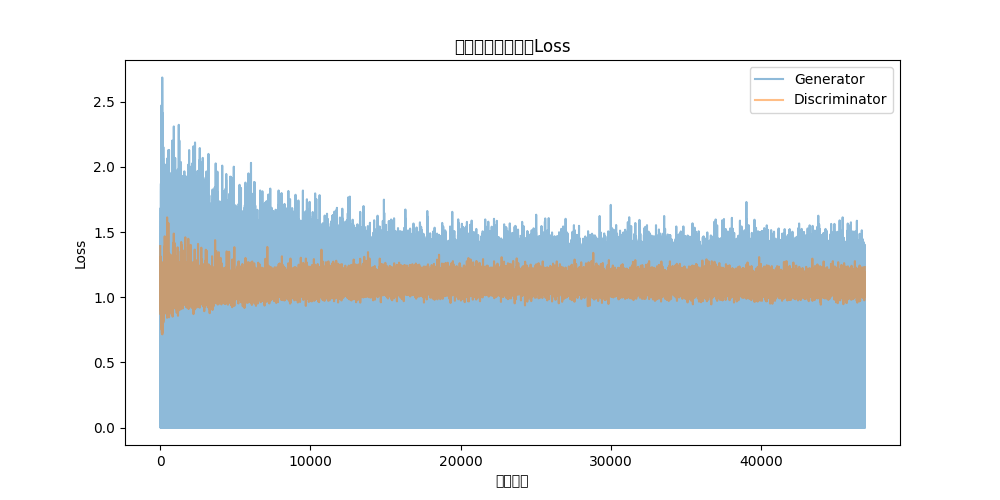
\includegraphics[width=0.8\textwidth]{loss_curves.png}
\caption{原始GAN训练损失曲线}
\label{fig:loss_curves}
\end{figure}

\begin{itemize}
\item \textbf{训练初期}:判别器损失快速下降,生成器损失上升,表明判别器在初期占据优势
\item \textbf{训练中期}:两个网络的损失趋于平衡,出现振荡现象,这是GAN训练的典型特征
\item \textbf{训练后期}:损失逐渐稳定,但仍存在一定的波动,说明两个网络达到了动态平衡
\end{itemize}

图\ref{fig:dcgan_curves}展示了DCGAN模型的训练损失曲线:

\begin{figure}[H]
\centering
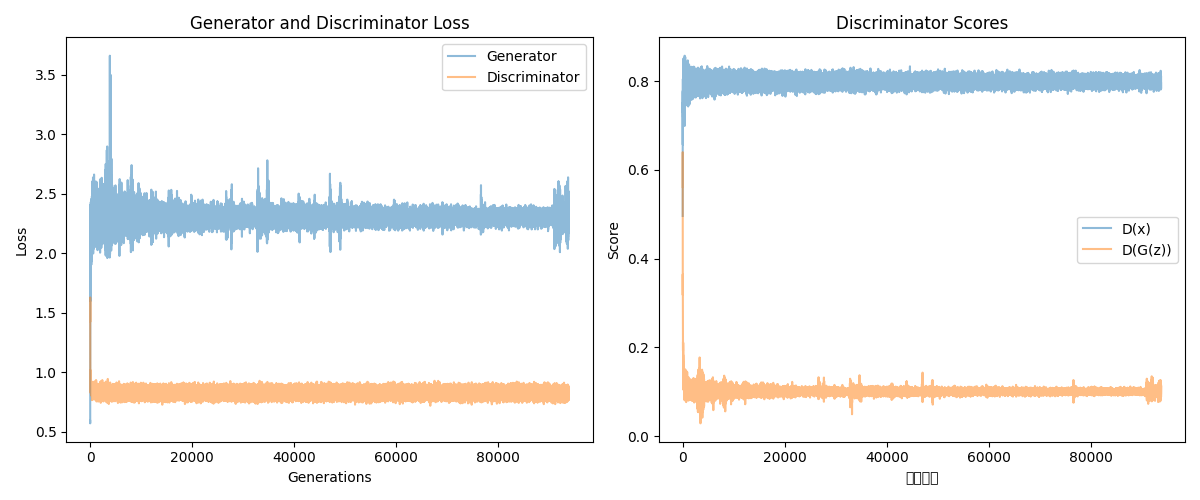
\includegraphics[width=0.8\textwidth]{training_curves.png}
\caption{DCGAN训练损失曲线}
\label{fig:dcgan_curves}
\end{figure}

相比原始GAN,DCGAN的训练过程更加稳定,损失波动较小,收敛速度更快。

\subsection{生成图像质量分析}

\subsubsection{原始GAN生成效果}

图\ref{fig:gan_progression}展示了原始GAN在不同训练阶段的生成效果:

\begin{figure}[H]
\centering
\subfigure[第0轮]{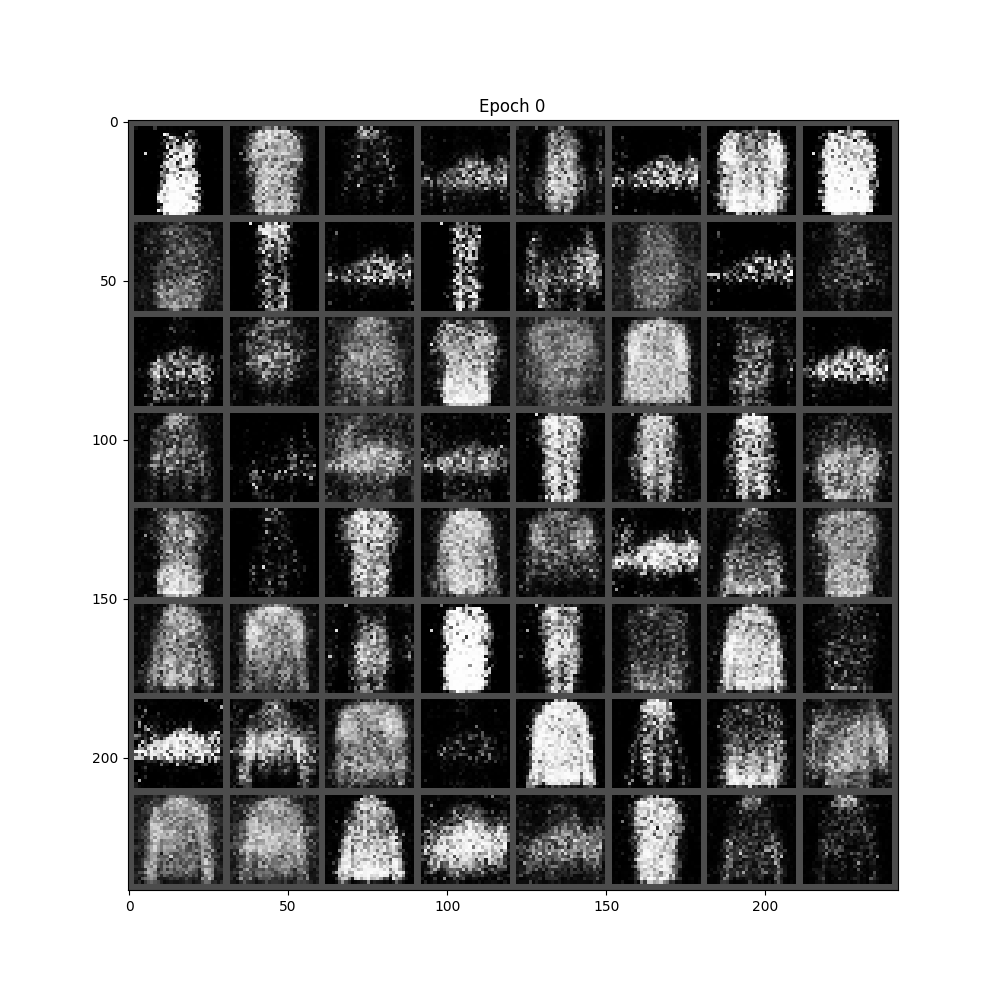
\includegraphics[width=0.3\textwidth]{fake_epoch_0.png}}
\subfigure[第25轮]{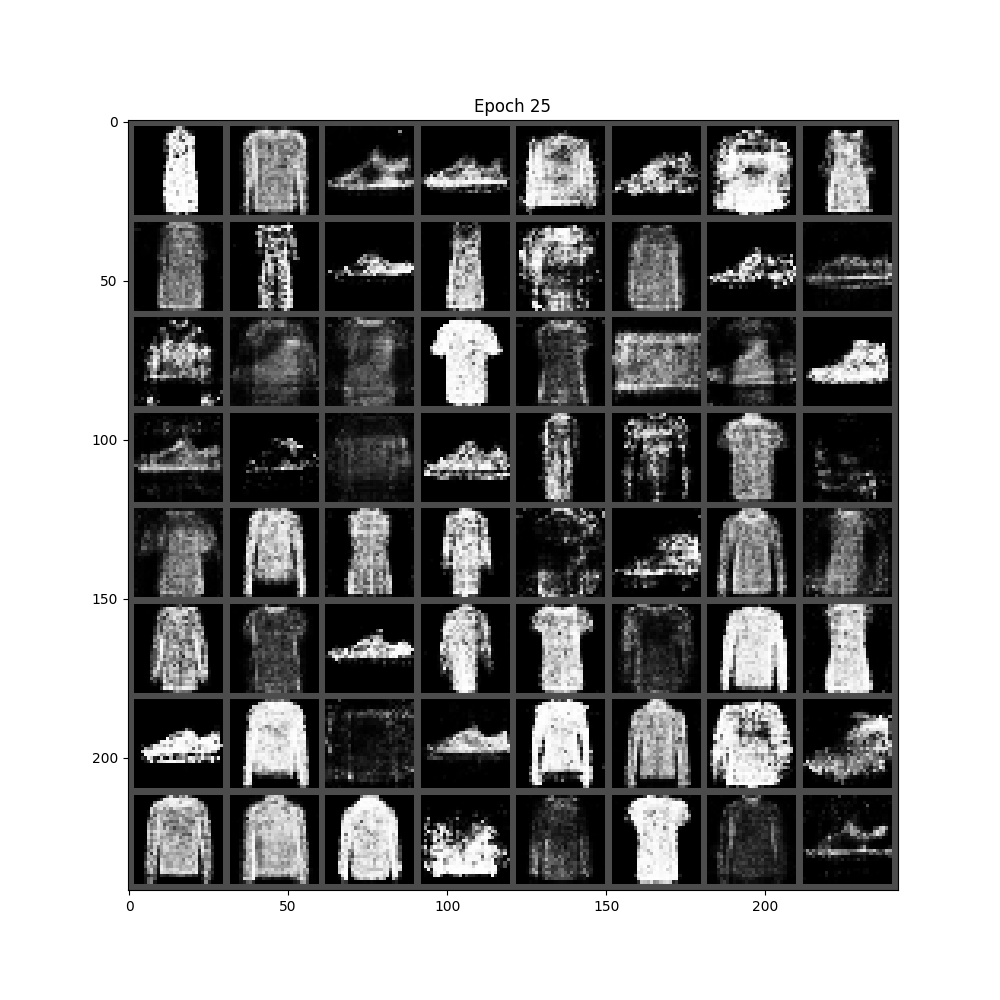
\includegraphics[width=0.3\textwidth]{fake_epoch_25.png}}
\subfigure[第49轮]{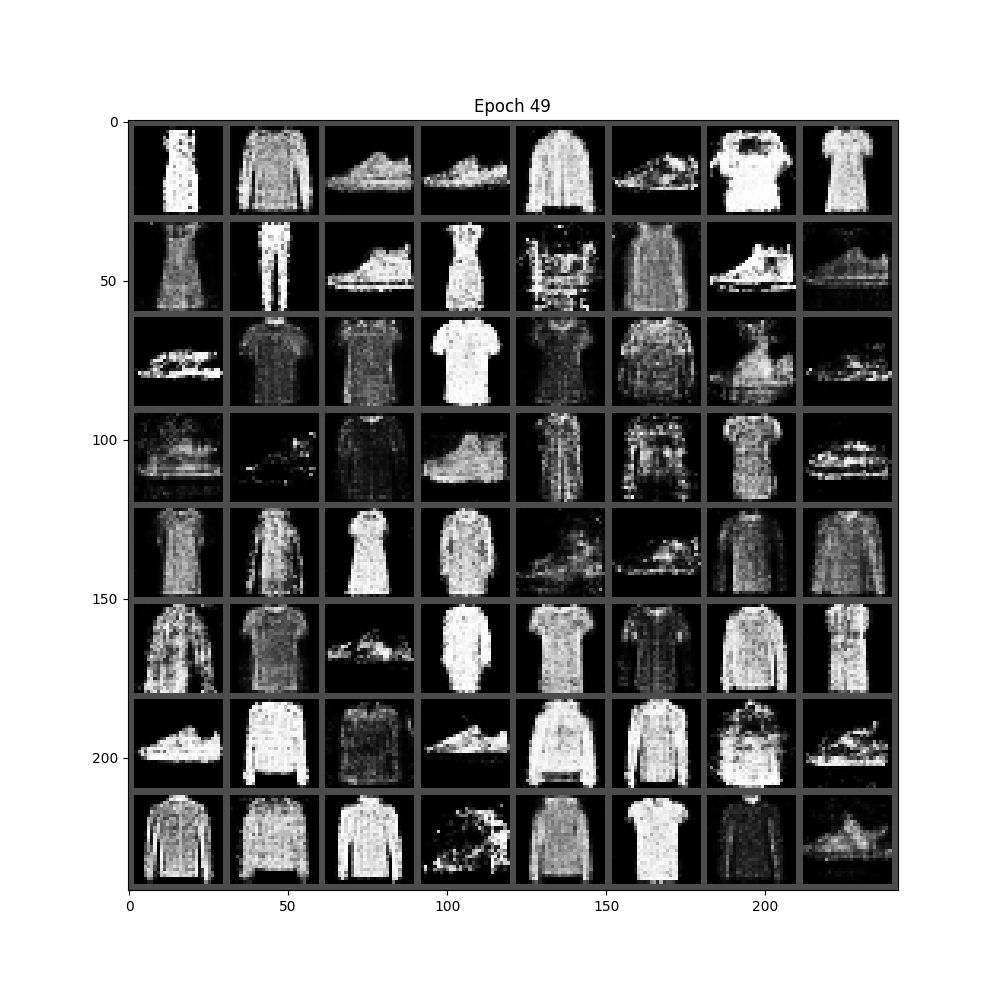
\includegraphics[width=0.3\textwidth]{fake_epoch_49.png}}
\caption{原始GAN训练过程中的生成图像}
\label{fig:gan_progression}
\end{figure}

从生成效果可以看出:
\begin{itemize}
\item \textbf{训练初期}:生成的图像模糊不清,缺乏明确的结构
\item \textbf{训练中期}:图像质量有所改善,开始出现服装的轮廓
\item \textbf{训练后期}:生成的图像更加清晰,能够识别出不同类型的服装
\end{itemize}

\subsubsection{DCGAN生成效果}

图\ref{fig:dcgan_progression}展示了DCGAN在不同训练阶段的生成效果:

\begin{figure}[H]
\centering
\subfigure[第0轮]{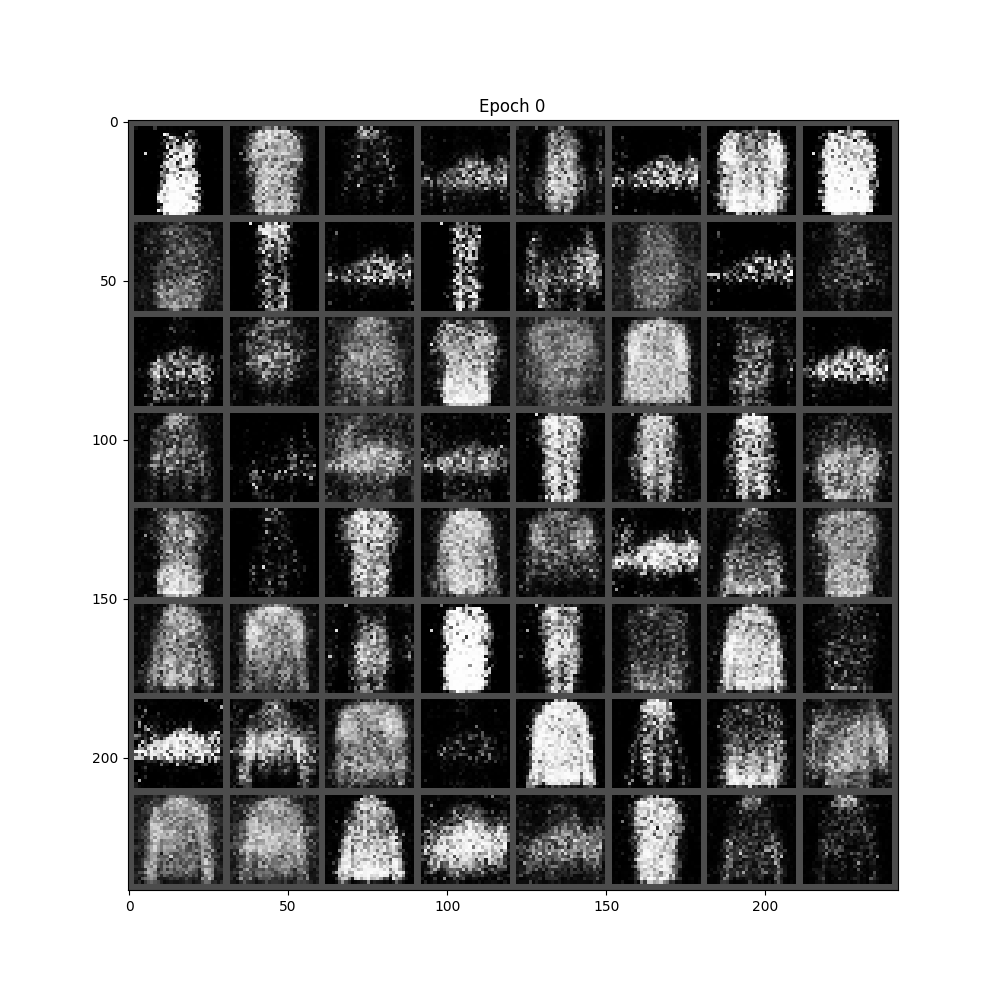
\includegraphics[width=0.3\textwidth]{fake_epoch_0.png}}
\subfigure[第25轮]{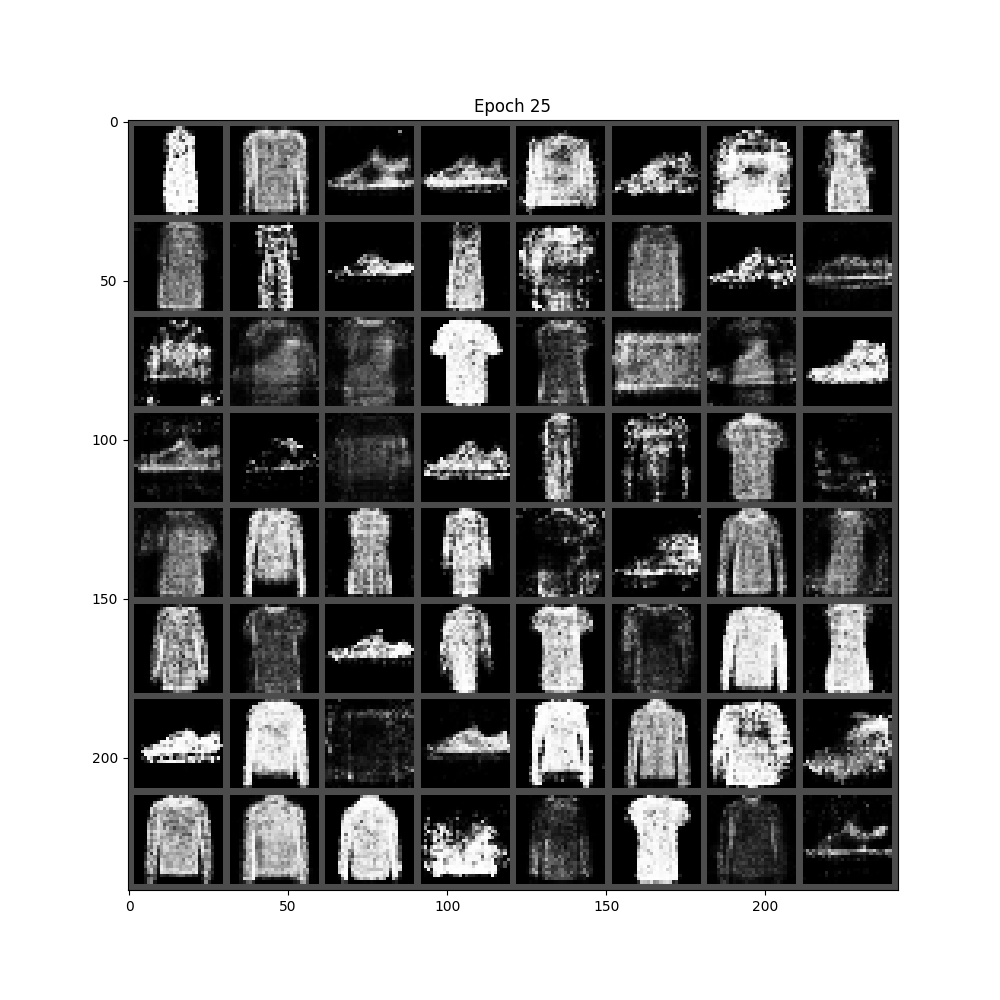
\includegraphics[width=0.3\textwidth]{fake_epoch_25.png}}
\subfigure[第49轮]{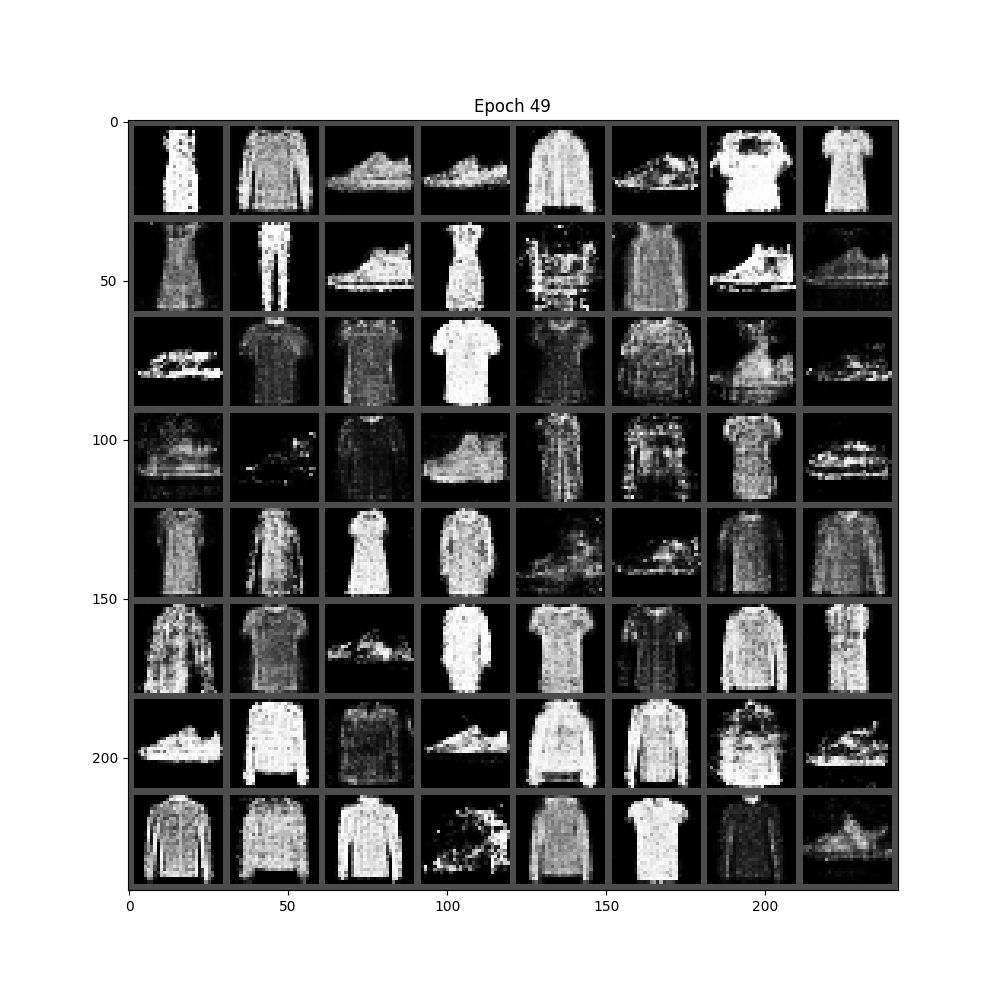
\includegraphics[width=0.3\textwidth]{fake_epoch_49.png}}
\caption{DCGAN训练过程中的生成图像}
\label{fig:dcgan_progression}
\end{figure}

DCGAN的生成效果明显优于原始GAN:
\begin{itemize}
\item \textbf{图像清晰度}:DCGAN生成的图像更加清晰,细节更丰富
\item \textbf{结构完整性}:服装的形状和结构更加完整和真实
\item \textbf{多样性}:能够生成多种不同类型的服装图像
\end{itemize}

\subsection{潜在空间探索}

为了分析生成器学到的潜在表示,我们对潜在空间进行了探索。通过固定随机向量的大部分维度,只改变特定维度的值,观察生成图像的变化。

\begin{figure}[H]
\centering
\subfigure[维度4的变化]{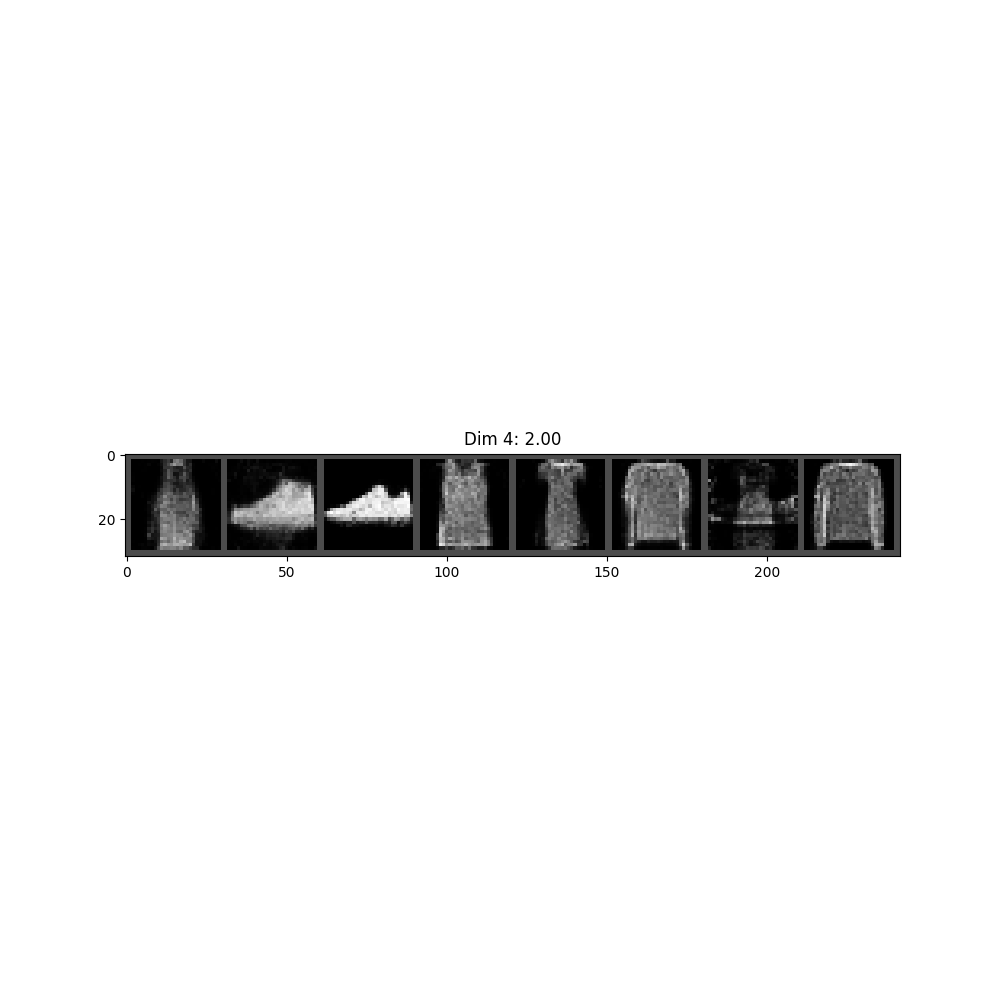
\includegraphics[width=0.45\textwidth]{latent_dim_4_analysis.png}}
\subfigure[维度21的变化]{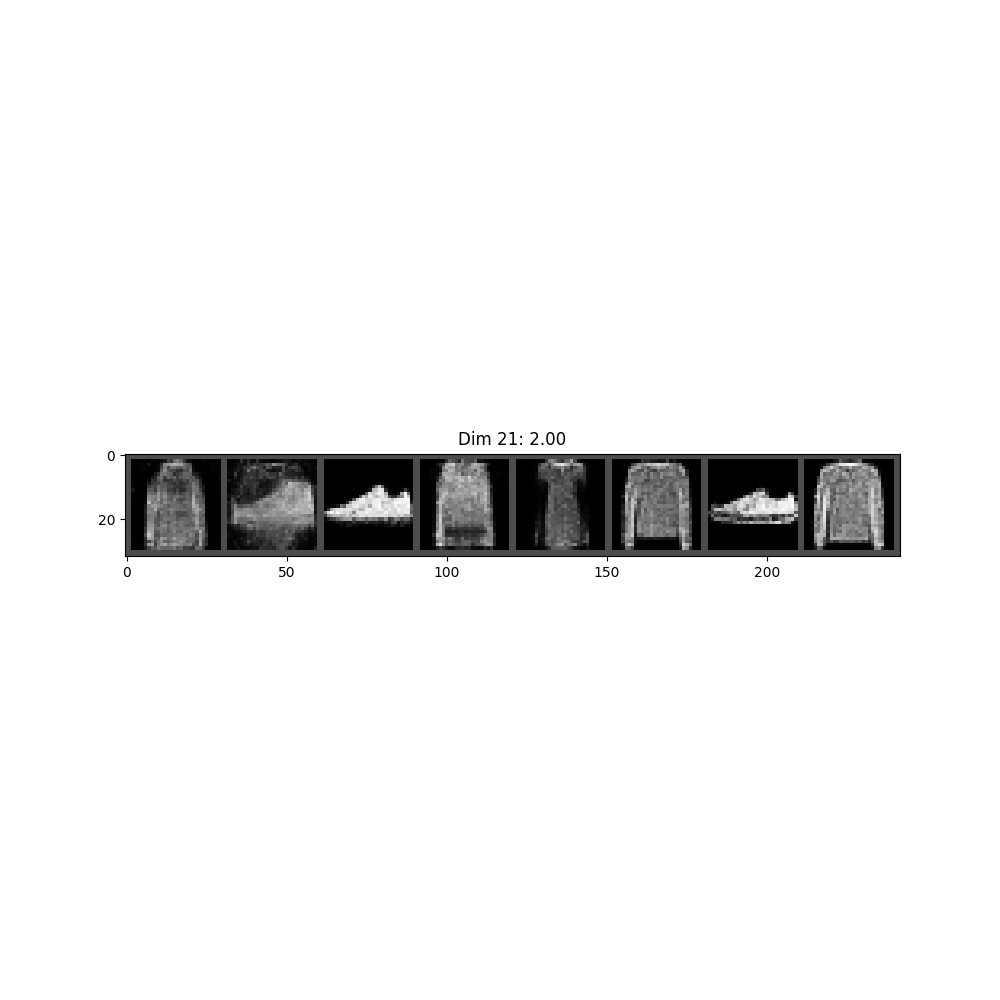
\includegraphics[width=0.45\textwidth]{latent_dim_21_analysis.png}}
\caption{潜在空间不同维度的影响分析}
\label{fig:latent_analysis}
\end{figure}

从潜在空间分析可以发现:
\begin{itemize}
\item \textbf{语义连续性}:改变潜在向量的特定维度会导致生成图像的连续变化
\item \textbf{特征控制}:不同维度控制着不同的视觉特征,如形状、纹理、亮度等
\item \textbf{插值效果}:在潜在空间中进行插值可以生成平滑过渡的图像序列
\end{itemize}

\subsection{性能对比分析}

\begin{table}[H]
\centering
\caption{原始GAN与DCGAN性能对比}
\begin{tabular}{|c|c|c|}
\hline
\textbf{评估指标} & \textbf{原始GAN} & \textbf{DCGAN} \\
\hline
训练稳定性 & 中等 & 高 \\
\hline
收敛速度 & 较慢 & 较快 \\
\hline
图像清晰度 & 中等 & 高 \\
\hline
模式崩塌风险 & 高 & 低 \\
\hline
计算复杂度 & 低 & 中等 \\
\hline
参数数量 & 较少 & 较多 \\
\hline
\end{tabular}
\end{table}

%--------------------------实验心得-------------------------------
\section{实验心得}

\subsection{主要收获}

通过本次GAN实验,我获得了以下主要收获:

\begin{enumerate}
\item \textbf{理论理解}:深入理解了生成对抗网络的基本原理和训练机制,掌握了生成器和判别器的对抗训练过程
\item \textbf{实践能力}:熟练掌握了PyTorch框架下GAN模型的实现,包括网络架构设计、损失函数定义、训练循环编写等
\item \textbf{调试技巧}:学会了GAN训练中的常见问题及解决方法,如模式崩塌、训练不稳定等
\item \textbf{评估方法}:了解了生成模型的评估方法,包括定性分析和定量指标
\end{enumerate}

\subsection{技术难点与解决方案}

\begin{itemize}
\item \textbf{训练不稳定}:通过调整学习率、使用标签平滑、添加噪声等技术提高训练稳定性
\item \textbf{模式崩塌}:采用不同的网络架构、正则化技术和训练策略来缓解模式崩塌问题
\item \textbf{超参数调优}:通过实验对比找到最适合的学习率、批次大小等超参数
\end{itemize}

\subsection{改进方向}

未来可以从以下几个方向进一步改进:

\begin{enumerate}
\item \textbf{网络架构}:尝试更先进的GAN变体,如WGAN、LSGAN、StyleGAN等
\item \textbf{损失函数}:探索不同的损失函数设计,提高训练稳定性和生成质量
\item \textbf{评估指标}:引入更客观的评估指标,如FID、IS等
\item \textbf{应用扩展}:将GAN应用到更复杂的任务中,如图像编辑、风格迁移等
\end{enumerate}

%--------------------------结论-------------------------------
\section{结论}

本实验成功实现了原始GAN和DCGAN两种生成对抗网络模型,并在FashionMNIST数据集上进行了训练和评估。实验结果表明:

\begin{enumerate}
\item \textbf{DCGAN优势明显}:相比原始GAN,DCGAN在图像生成质量、训练稳定性和收敛速度方面都有显著提升
\item \textbf{卷积结构的重要性}:卷积神经网络结构能够更好地捕捉图像的空间特征,生成更加逼真的图像
\item \textbf{潜在空间的可解释性}:通过潜在空间探索,发现生成器学到了有意义的特征表示
\item \textbf{训练技巧的重要性}:合适的网络架构设计、超参数设置和训练策略对GAN的成功训练至关重要
\end{enumerate}

本实验为深入理解生成对抗网络提供了宝贵的实践经验,为后续研究更先进的生成模型奠定了基础。

%--------------------------附录-------------------------------
\appendix
\section{附录:代码实现}

\subsection{原始GAN模型实现}

\begin{lstlisting}[language=Python, caption=原始GAN生成器和判别器]
import torch
import torch.nn as nn

class Generator(nn.Module):
    def __init__(self, z_dim=100):
        super(Generator, self).__init__()
        # 改进的生成器架构 - 增加深度和BatchNorm
        self.fc1 = nn.Linear(z_dim, 256)
        self.bn1 = nn.BatchNorm1d(256)
        self.fc2 = nn.Linear(256, 512)
        self.bn2 = nn.BatchNorm1d(512)
        self.fc3 = nn.Linear(512, 1024)
        self.bn3 = nn.BatchNorm1d(1024)
        self.fc4 = nn.Linear(1024, 784)  # 28*28=784
        self.leaky_relu = nn.LeakyReLU(0.2)
        self.dropout = nn.Dropout(0.3)

    def forward(self, x):
        # 实现改进的生成器
        x = self.leaky_relu(self.bn1(self.fc1(x)))
        x = self.dropout(x)
        x = self.leaky_relu(self.bn2(self.fc2(x)))
        x = self.dropout(x)
        x = self.leaky_relu(self.bn3(self.fc3(x)))
        x = self.dropout(x)
        out = self.fc4(x)
        
        out = torch.tanh(out) # range [-1, 1]
        # convert to image 
        out = out.view(out.size(0), 1, 28, 28)
        return out

class Discriminator(torch.nn.Module):
    def __init__(self, inp_dim=784):
        super(Discriminator, self).__init__()
        # 改进的判别器架构 - 增加深度和Dropout
        self.fc1 = torch.nn.Linear(inp_dim, 1024)
        self.fc2 = torch.nn.Linear(1024, 512)
        self.fc3 = torch.nn.Linear(512, 256)
        self.fc4 = torch.nn.Linear(256, 1)
        self.leaky_relu = torch.nn.LeakyReLU(0.2)
        self.dropout = torch.nn.Dropout(0.3)
        self.sigmoid = torch.nn.Sigmoid()
        
    def forward(self, x):
        x = x.view(x.size(0), 784) # flatten
        # 实现改进的判别器
        x = self.leaky_relu(self.fc1(x))
        x = self.dropout(x)
        x = self.leaky_relu(self.fc2(x))
        x = self.dropout(x)
        x = self.leaky_relu(self.fc3(x))
        x = self.dropout(x)
        x = self.sigmoid(self.fc4(x))
        return x
\end{lstlisting}

\subsection{DCGAN模型实现}

\begin{lstlisting}[language=Python, caption=DCGAN生成器和判别器]
class Generator(nn.Module):
    def __init__(self, z_dim=100, ngf=64):
        super(Generator, self).__init__()
        self.z_dim = z_dim
        
        self.main = nn.Sequential(
            # 输入: z_dim x 1 x 1
            nn.ConvTranspose2d(z_dim, ngf * 8, 4, 1, 0, bias=False),
            nn.BatchNorm2d(ngf * 8),
            nn.ReLU(True),
            # 状态大小: (ngf*8) x 4 x 4
            
            nn.ConvTranspose2d(ngf * 8, ngf * 4, 4, 2, 1, bias=False),
            nn.BatchNorm2d(ngf * 4),
            nn.ReLU(True),
            # 状态大小: (ngf*4) x 7 x 7
            
            nn.ConvTranspose2d(ngf * 4, ngf * 2, 4, 2, 1, bias=False),
            nn.BatchNorm2d(ngf * 2),
            nn.ReLU(True),
            # 状态大小: (ngf*2) x 14 x 14
            
            nn.ConvTranspose2d(ngf * 2, ngf, 4, 2, 1, bias=False),
            nn.BatchNorm2d(ngf),
            nn.ReLU(True),
            # 状态大小: ngf x 28 x 28
            
            nn.Conv2d(ngf, 1, 3, 1, 1, bias=False),
            nn.Tanh()
            # 输出状态大小: 1 x 28 x 28
        )
        
        self.apply(self._weights_init)
    
    def _weights_init(self, m):
        classname = m.__class__.__name__
        if classname.find('Conv') != -1:
            nn.init.normal_(m.weight.data, 0.0, 0.02)
        elif classname.find('BatchNorm') != -1:
            nn.init.normal_(m.weight.data, 1.0, 0.02)
            nn.init.constant_(m.bias.data, 0)
    
    def forward(self, input):
        if input.dim() == 2:
            input = input.view(input.size(0), input.size(1), 1, 1)
        return self.main(input)

class Discriminator(nn.Module):
    def __init__(self, ndf=64):
        super(Discriminator, self).__init__()
        
        self.main = nn.Sequential(
            # 输入: 1 x 28 x 28
            nn.Conv2d(1, ndf, 4, 2, 1, bias=False),
            nn.LeakyReLU(0.2, inplace=True),
            nn.Dropout2d(0.3),
            
            nn.Conv2d(ndf, ndf * 2, 4, 2, 1, bias=False),
            nn.BatchNorm2d(ndf * 2),
            nn.LeakyReLU(0.2, inplace=True),
            nn.Dropout2d(0.3),
            
            nn.Conv2d(ndf * 2, ndf * 4, 4, 2, 1, bias=False),
            nn.BatchNorm2d(ndf * 4),
            nn.LeakyReLU(0.2, inplace=True),
            nn.Dropout2d(0.3),
            
            nn.Conv2d(ndf * 4, 1, 3, 1, 0, bias=False),
            nn.Sigmoid()
        )
        
        self.apply(self._weights_init)
    
    def _weights_init(self, m):
        classname = m.__class__.__name__
        if classname.find('Conv') != -1:
            nn.init.normal_(m.weight.data, 0.0, 0.02)
        elif classname.find('BatchNorm') != -1:
            nn.init.normal_(m.weight.data, 1.0, 0.02)
            nn.init.constant_(m.bias.data, 0)
    
    def forward(self, input):
        return self.main(input).view(-1, 1).squeeze(1)
\end{lstlisting}

\subsection{改进的卷积GAN模型实现}

\begin{lstlisting}[language=Python, caption=改进的卷积GAN生成器和判别器]
import torch
import torch.nn as nn

class Generator(nn.Module):
    def __init__(self, z_dim=100, ngf=64):
        """
        改进的DCGAN生成器
        z_dim: 输入噪声维度
        ngf: 生成器特征图数量
        """
        super(Generator, self).__init__()
        self.z_dim = z_dim
        
        # 输入是一个z_dim维的噪声向量,输出是(1, 28, 28)的图像
        # 确保输出大小正好是28x28
        
        self.main = nn.Sequential(
            # 输入: z_dim x 1 x 1
            # 第一层:转置卷积,将1x1扩展到4x4
            nn.ConvTranspose2d(z_dim, ngf * 8, 4, 1, 0, bias=False),
            nn.BatchNorm2d(ngf * 8),
            nn.ReLU(True),
            # 状态大小: (ngf*8) x 4 x 4
            
            # 第二层:4x4 -> 7x7
            nn.ConvTranspose2d(ngf * 8, ngf * 4, 4, 2, 1, bias=False),
            nn.BatchNorm2d(ngf * 4),
            nn.ReLU(True),
            # 状态大小: (ngf*4) x 7 x 7
            
            # 第三层:7x7 -> 14x14
            nn.ConvTranspose2d(ngf * 4, ngf * 2, 4, 2, 1, bias=False),
            nn.BatchNorm2d(ngf * 2),
            nn.ReLU(True),
            # 状态大小: (ngf*2) x 14 x 14
            
            # 第四层:14x14 -> 28x28 (精确匹配FashionMNIST大小)
            nn.ConvTranspose2d(ngf * 2, ngf, 4, 2, 1, bias=False),
            nn.BatchNorm2d(ngf),
            nn.ReLU(True),
            # 状态大小: ngf x 28 x 28
            
            # 最后一层:保持28x28大小不变,只改变通道数
            nn.Conv2d(ngf, 1, 3, 1, 1, bias=False),
            nn.Tanh()
            # 输出状态大小: 1 x 28 x 28
        )
        
        # 权重初始化
        self.apply(self._weights_init)
    
    def _weights_init(self, m):
        """权重初始化函数"""
        classname = m.__class__.__name__
        if classname.find('Conv') != -1:
            nn.init.normal_(m.weight.data, 0.0, 0.02)
        elif classname.find('BatchNorm') != -1:
            nn.init.normal_(m.weight.data, 1.0, 0.02)
            nn.init.constant_(m.bias.data, 0)
    
    def forward(self, input):
        # 将输入reshape为适合卷积的形状
        if input.dim() == 2:
            input = input.view(input.size(0), input.size(1), 1, 1)
        return self.main(input)

class Discriminator(nn.Module):
    def __init__(self, ndf=64):
        """
        改进的DCGAN判别器
        ndf: 判别器特征图数量
        """
        super(Discriminator, self).__init__()
        
        self.main = nn.Sequential(
            # 输入: 1 x 28 x 28
            # 第一层:28x28 -> 14x14
            nn.Conv2d(1, ndf, 4, 2, 1, bias=False),
            nn.LeakyReLU(0.2, inplace=True),
            nn.Dropout2d(0.3),  # 增加dropout比例
            # 状态大小: ndf x 14 x 14
            
            # 第二层:14x14 -> 7x7
            nn.Conv2d(ndf, ndf * 2, 4, 2, 1, bias=False),
            nn.BatchNorm2d(ndf * 2),
            nn.LeakyReLU(0.2, inplace=True),
            nn.Dropout2d(0.3),  # 增加dropout比例
            # 状态大小: (ndf*2) x 7 x 7
            
            # 第三层:7x7 -> 4x4
            nn.Conv2d(ndf * 2, ndf * 4, 4, 2, 1, bias=False),
            nn.BatchNorm2d(ndf * 4),
            nn.LeakyReLU(0.2, inplace=True),
            nn.Dropout2d(0.3),  # 增加dropout比例
            # 状态大小: (ndf*4) x 4 x 4
            
            # 第四层:4x4 -> 1x1
            # 使用3x3卷积核和padding=0,确保能处理3x3的输入
            nn.Conv2d(ndf * 4, 1, 3, 1, 0, bias=False),
            nn.Sigmoid()
            # 输出状态大小: 1 x 1 x 1
        )
        
        # 权重初始化
        self.apply(self._weights_init)
    
    def _weights_init(self, m):
        """权重初始化函数"""
        classname = m.__class__.__name__
        if classname.find('Conv') != -1:
            nn.init.normal_(m.weight.data, 0.0, 0.02)
        elif classname.find('BatchNorm') != -1:
            nn.init.normal_(m.weight.data, 1.0, 0.02)
            nn.init.constant_(m.bias.data, 0)
    
    def forward(self, input):
        output = self.main(input)
        # 确保输出形状与标签匹配
        # 首先打平输出,然后确保长度与批次大小匹配
        batch_size = input.size(0)
        # 计算每个样本的平均值,确保输出形状为 [batch_size]
        return output.view(batch_size, -1).mean(dim=1)
\end{lstlisting}

\subsection{训练代码}

\begin{lstlisting}[language=Python, caption=GAN训练循环]
def train_gan(num_epochs=50, batch_size=64, lr=0.0002, beta1=0.5):
    device = torch.device('cuda' if torch.cuda.is_available() else 'cpu')
    
    # 数据加载
    transform = transforms.Compose([
        transforms.ToTensor(),
        transforms.Normalize((0.5,), (0.5,))
    ])
    
    dataset = datasets.FashionMNIST(
        root='../FashionMNIST/',
        transform=transform,
        download=True
    )
    dataloader = torch.utils.data.DataLoader(
        dataset, batch_size=batch_size, shuffle=True
    )
    
    # 初始化模型
    G = Generator().to(device)
    D = Discriminator().to(device)
    
    # 优化器
    optimizerD = torch.optim.Adam(D.parameters(), lr=lr, betas=(beta1, 0.999))
    optimizerG = torch.optim.Adam(G.parameters(), lr=lr, betas=(beta1, 0.999))
    
    # 损失函数
    criterion = nn.BCELoss()
    
    # 训练循环
    for epoch in range(num_epochs):
        for i, (real_imgs, _) in enumerate(dataloader):
            batch_size = real_imgs.size(0)
            
            # 训练判别器
            D.zero_grad()
            real_imgs = real_imgs.to(device)
            real_label = torch.ones(batch_size, 1).to(device) * 0.9
            fake_label = torch.zeros(batch_size, 1).to(device) + 0.1
            
            output_real = D(real_imgs)
            d_loss_real = criterion(output_real, real_label)
            
            noise = torch.randn(batch_size, 100, device=device)
            fake_imgs = G(noise)
            output_fake = D(fake_imgs.detach())
            d_loss_fake = criterion(output_fake, fake_label)
            
            d_loss = d_loss_real + d_loss_fake
            d_loss.backward()
            optimizerD.step()
            
            # 训练生成器
            if i % 2 == 0:
                G.zero_grad()
                noise = torch.randn(batch_size, 100, device=device)
                fake_imgs = G(noise)
                output_fake = D(fake_imgs)
                g_loss = criterion(output_fake, torch.ones(batch_size, 1).to(device))
                g_loss.backward()
                optimizerG.step()
\end{lstlisting}

\end{document}
 

\end{document}